\documentclass[../../main.tex]{subfiles}
\begin{document}
\tracingall

% Fluid simulation
% SPH 
% PCISPH
% Our contribution

%%%%%%%%
\section{Fluid simulation}
%%%%%%%%
In the field of computer graphics, realistic looking scenes 
%and terrain
has always been desired. When it comes to fluid simulation there are multiple approaches to achieve realistic looking liquids. For the most part, the time cost associated with a realistic simulations is high. Therefore, much research has been devoted to reduce total computational time. Methods for doing so are usually divided into three subgroups: Eulerian, Lagrangian, and a combination of Eulerian and Lagrangian.

%Navier stokes?

%With the increasing performance and memory capacity of computers, most areas are getting closer to being indistinguishable from reality. However, realistic looking fluid animation is still an area which is too computationally heavy to use efficiently(not implicit). There are multiple approaches with varying positive key aspects, they range in complexity from computationally expensive, high quality animations, towards simpler real-time systems. 

%Some kind of important-word list
%Advection:



Eulerian, or grid-based, methods are a common choice for simulating fluids in the industry due to high coherence with the ground reality. In Eulerian methods physical quantities (pressure, density, velocity, and so on) of the fluid are defined on a grid and are then changed over time, but the grid remains fixed. This can be visualized as observing a river pass by while sitting at the riverbank; properties of constant points in the water change continuously, but the observed position remains the same. 

Lagrangian methods, as opposed to the Eulerian, move fluid mass around explicitly. The quantities are tied to a small part of the fluid which is tracked through the whole simulation. An analogy would be sitting in a boat and drifting down a river while watching the water around the boat. These methods are usually more computationally expensive because parcel of fluid needs to be directly aware of its surroundings which requires expensive neighborhood calculations. On the other hand, they offer advantages on simulating small scale features like droplets and splashes, because the surface is not bound to a grid but is instead built from whichever particles are visible. In addition, Lagrangian methods conserve mass implicitly and do not need a separate scheme for mass conservation. 
% Mention that the number of particles is very important for the computational cost

Whether a simulation method is Eulerian or Lagrangian, it is forwarded with a time step, a small value which is classically chosen globally and do not vary throughout the simulation. The time step determines how far the simulation is forwarded in each iteration. A larger time step forwards the flow of the fluid further, and thus decreases the required total computational time. Although a large time step seems desirable, choosing it too large could, for instance, cause two particles in the fluid to be forwarded in such a way that they occupy the same space. This can cause physically incorrect movement and displeasing visual results and is referred to as instability or unstable simulation.

It is, however, still desirable to have as large as possible value for the time step but still maintain a stable simulation. While the total computational time changes, the time for each iteration stays the same. This implies that a simulation that uses a large time step can be simulated further with the same computational cost compared to the same simulation using a lower time step. Such a decrease in computational time is desirable and is what many techniques for simulating fluid seek to achieve.


%%%%%%%%
\section{Smooth Particles Hydrodynamics}
%%%%%%%%
Our work is based on a variant of a Lagrangian method called \textit{Smooth Particles Hydrodynamics} (SPH), as the name implies SPH uses particles to simulate fluids. Each particle uses the distance to its neighbours to calculate a density value, this value is then used to compute the forward force and velocity. The new position is calculated by forwarding every particle's current position a small distance, using its velocity and a given time step. 

It is important to make sure that particles do not end up inside each other after an iteration, as doing so leads to undesirable visual effects and may even introduce instability. This limitation is called incompressibility and most liquids in computer graphics are approximated to be fully incompressible. The standard SPH method \citep{lucy1977numerical} does not enforce incompressibility so in an attempt to do so, Becker and Teschner introduced Weakly Compressible SPH (WCSPH) \citep{becker2007weakly}. While this method enforced near-incompressibility it came with a time step restriction which required a low time step to stay stable.

To increase the time step Solenthaler and Pajarola developed a Predictive-Corrective Incompressible SPH (PCISPH) \citep{solenthaler2009predictive}. By using larger time step their approach could simulate further with less total computational time. This, however, introduced aforementioned errors in density, and thus made the entire simulation unstable. They solved this by introducing an additional step in the algorithm which predicts each particle's new position and iteratively applies a correction force if the density is over a certain threshold. The correction force is then used to calculate the particle's actual new position. Although this would lead to each iteration being more expensive when compared to WCSPH, a significant speedup is achieved because the time step can be many times larger.

To further decrease total computation time Solenthaler also introduced the Two-scale Resolution method \citep{solenthaler2011two}. This method uses two separate simulation with different particle sizes. The particles in one simulation only interacts indirectly with the particles in the other. One simulation uses larger (and therefore a smaller amount of) particles and the other simulation uses smaller particles but in a limited area. This area is a subset of the whole simulation where details are more important. Since the rest of the simulation requires fewer particles and therefore less computations, a speedup is achieved. 

In contrast to reducing the number of particles, Regional Time Stepping by \citet{goswami2014regional} reduces computation time by using varying time steps based on the amount of movement in each area. Particles in areas with with small movements are assigned larger time step and are therefore not required to update as often. On the other hand, particles in areas with high movement are assigned a smaller time step. Thus less computational time is spent on the parts that exhibits less complexity.

Seeing as the two-scale resolution and regional time stepping methods improve on two different aspects of the PCISPH technique, we propose a method combining the two. Our method, like two scale, uses two simulations both of which individually calculates what time steps to use in which regions, in the same way as RTS. 
%Our method uses two simulations which calculates what time step to use in which regions individually.

%\begin{figure}[h]
%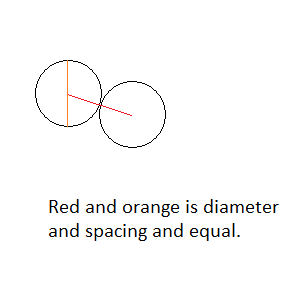
\includegraphics{image/spacing.png}
%\caption[Test image]{An image depicting the relationship between particle size and particle spacing.}     
%\label{fig:spacing}
%\end{figure}
\end{document}